\let\negmedspace\undefined
\let\negthickspace\undefined
\documentclass[journal]{IEEEtran}
\usepackage[a5paper, margin=10mm, onecolumn]{geometry}
%\usepackage{lmodern} % Ensure lmodern is loaded for pdflatex
\usepackage{tfrupee} % Include tfrupee package

\setlength{\headheight}{1cm} % Set the height of the header box
\setlength{\headsep}{0mm}     % Set the distance between the header box and the top of the text

\usepackage{gvv-book}
\usepackage{gvv}
\usepackage{cite}
\usepackage{amsmath,amssymb,amsfonts,amsthm}
\usepackage{algorithmic}
\usepackage{graphicx}
\usepackage{textcomp}
\usepackage{xcolor}
\usepackage{txfonts}
\usepackage{listings}
\usepackage{enumitem}
\usepackage{mathtools}
\usepackage{gensymb}
\usepackage{comment}
%\usepackage{multiclo}
\usepackage[breaklinks=true]{hyperref}
\usepackage{tkz-euclide} 
\usepackage{listings}
% \usepackage{gvv} 
\graphicspath{ {./figs/} }

\begin{document}


\title{
ASSIGNMENT 4: GATE 2019 \\
MN:MINING ENGINEERING}
\author{AI25BTECH11010 - Dhanush Kumar}
\maketitle
\renewcommand{\thefigure}{\theenumi}
\renewcommand{\thetable}{\theenumi}


\begin{enumerate}

\item John Thomas, an  \underline{\hspace{2cm}} writer, passed away in 2018.

	\hfill(GATE MN 2019)
\begin{multicols}{2}
\begin{enumerate}
\item imminent  
\item prominent  
\item eminent  
\item dominant  
\end{enumerate}
\end{multicols}


\item  \underline{\hspace{2cm}} I permitted him to leave, I wouldn’t have had any problem with him being absent,  \underline{\hspace{2cm}} I?

\hfill(GATE MN 2019)
\begin{multicols}{2}
\begin{enumerate}
\item Had, wouldn’t  
\item Have, would  
\item Had, would  
\item Have, wouldn’t  
\end{enumerate}
\end{multicols}

\item A worker noticed that the hour hand on the factory clock had moved by 225 degrees during her stay at the factory. For how long did she stay in the factory?

	\hfill(GATE MN 2019)
\begin{multicols}{2}
\begin{enumerate}
\item 3.75 hours  
\item 4 hours and 15 mins  
\item 8.5 hours  
\item 7.5 hours  
\end{enumerate}
\end{multicols}


\item The sum and product of two integers are 26 and 165 respectively. The difference between these two integers is  \underline{\hspace{2cm}}.

	\hfill(GATE MN 2019)
\begin{multicols}{4}
\begin{enumerate}
\item 2  
\item 3  
\item 4  
\item 6  
\end{enumerate}
\end{multicols}


\item The minister avoided any mention of the issue of women’s reservation in the private sector. He was accused of  \underline{\hspace{2cm}} the issue.

	\hfill(GATE MN 2019)
\begin{multicols}{4}
\begin{enumerate}
\item collaring  
\item skirting  
\item tying  
\item belting  
\end{enumerate}
\end{multicols}

\item Under a certain legal system, prisoners are allowed to make one statement. If their statement turns out to be true then they are hanged. If the statement turns out to be false then they are shot. One prisoner made a statement and the judge had no option but to set him free. Which one of the following could be that statement?


	\hfill(GATE MN 2019)
\begin{enumerate}
\item I did not commit the crime  
\item I committed the crime  
\item I will be shot  
\item You committed the crime  
\end{enumerate}


\item A person divided an amount of Rs.\ 100,000 into two parts and invested in two different schemes. In one he got 10\% profit and in the other he got 12\%. If the profit percentages are interchanged with these investments he would have got Rs.\ 120 less. Find the ratio between his investments in the two schemes.

	\hfill(GATE MN 2019)
\begin{multicols}{4}
\begin{enumerate}
\item 9 : 16  
\item 11 : 14  
\item 37 : 63  
\item 47 : 53  
\end{enumerate}
\end{multicols}


\item Congo was named by Europeans. Congo’s dictator Mobuto later changed the name of the country and the river to Zaire with the objective of Africanising names of persons and spaces. However, the name Zaire was a Portuguese alteration of \textit{Nzadi o Nzere}, a local African term meaning ‘River that swallows Rivers’. Zaire was the Portuguese name for the Congo river in the 16th and 17th centuries.  

Which one of the following statements can be inferred from the paragraph above?

\hfill(GATE MN 2019)
\begin{enumerate}
\item Mobuto was not entirely successful in Africanising the name of his country  
\item The term \textit{Nzadi o Nzere} was of Portuguese origin  
\item Mobuto’s desire to Africanise names was prevented by the Portuguese  
\item As a dictator Mobuto ordered the Portuguese to alter the name of the river to Zaire  
\end{enumerate}

\item A firm hires employees at five different skill levels P, Q, R, S, T. 
The shares of employment at these skill levels of total employment in 2010 is given in the pie chart as shown. 
There were a total of 600 employees in 2010 and the total employment increased by 15\% from 2010 to 2016. 
The total employment at skill levels P, Q and R remained unchanged during this period. 
If the employment at skill level S increased by 40\% from 2010 to 2016, how many employees were there at skill level T in 2016?


\begin{figure}[H]                                
\centering
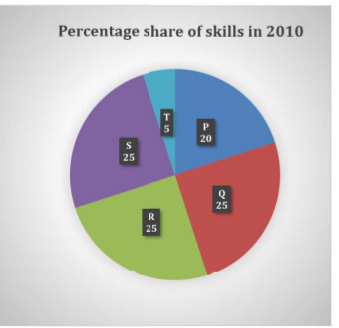
\includegraphics[width=0.5\textwidth]{Screenshot_2025_0818_124252.png}
\caption{}                                     
\label{fig:Q9}                             
\end{figure}


\hfill(GATE MN 2019)
\begin{multicols}{2}
\begin{enumerate}
\item 30
\item 35
\item 60
\item 72
\end{enumerate}
\end{multicols}


\item M and N had four children P, Q, R and S. Of them, only P and R were married. 
They had children X and Y respectively. If Y is a legitimate child of W, which one of the following statements is necessarily FALSE?


\hfill(GATE MN 2019)
\begin{multicols}{2}
\begin{enumerate}
\item M is the grandmother of Y
\item R is the father of Y
\item W is the wife of R
\item W is the wife of P
\end{enumerate}
\end{multicols}

\item Shear strength of rock joint is NOT dependent on

	\hfill(GATE MN 2019)
\begin{multicols}{2}
\begin{enumerate}
\item applied normal stress
\item applied shear stress
\item friction angle of the joint plane
\item cohesion of the joint plane
\end{enumerate}
\end{multicols}


\item If $f(x)$ is a polynomial function that passes through origin, and $g(x) = f'(x)$, then

	\hfill(GATE MN 2019)
\begin{multicols}{2}
\begin{enumerate}
\item $g(a) = f(a)$
\item $g(a) = f'(a)$
\item $\int_0^a g(x)dx = f(a)$
\item $\int_0^a f(x)dx = g(a)$
\end{enumerate}
\end{multicols}

\item A flat longwall panel is mined out at an area having subsidence factor $a$. 
The measured maximum subsidence on the surface is $S$ for a mining height of $m$. 
The subsidence is subcritical if

\hfill(GATE MN 2019)
\begin{multicols}{4}
\begin{enumerate}
\item $S = am$
\item $S = m/a$
\item $S > am$
\item $S < am$
\end{enumerate}
\end{multicols}

\item The PV diagram of four explosives is given below. 
The preferred explosive for adequate fragmentation in hard and brittle rock is
\begin{figure}[H]                                
\centering
	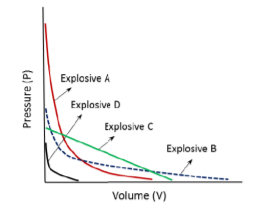
\includegraphics[width=0.5\textwidth]{Screenshot_2025_0818_123801.png}
\caption{}      
\label{fig:Q14}          
\end{figure}


\hfill(GATE MN 2019)
\begin{multicols}{2}
\begin{enumerate}

\item Explosive A
\item Explosive B
\item Explosive C
\item Explosive D
\end{enumerate}
\end{multicols}


\item As per classification of mineral resources “reserve” means


	\hfill(GATE MN 2019)
\begin{enumerate}
\item Identified resources
\item Identified and techno-economically viable resources
\item Hypothetical resources
\item Inferred resources
\end{enumerate}


\item If the sample statistic $\bar{X}$ is an unbiased estimator of the parameter $\mu$, then

	\hfill(GATE MN 2019)
\begin{multicols}{2}
\begin{enumerate}
\item $E(\mu - \bar{X}) = 0$
\item $E(\mu + \bar{X}) = 0$
\item $E(\mu - \bar{X})^2 = 0$
\item $E(\mu + \bar{X})^2 = 0$
\end{enumerate}
\end{multicols}

\item The vector sum of all the external forces acting on a rigid body is expressed as $\sum F$ and the vector sum of moments of the external forces about a point is given as $\sum M$. The rigid body is in equilibrium if

	\hfill(GATE MN 2019)
\begin{multicols}{2}
\begin{enumerate}
\item $\sum F - \sum M = 0$
\item $\sum F + \sum M = 0$
\item $\sum F = 0 \;\; \text{and} \;\; \sum M = 0$
\item $\sum F \neq 0 \;\; \text{and} \;\; \sum M = 0$
\end{enumerate}
\end{multicols}


\item For a regionalized variable $Z(x)$, at a lag distance $h$, the empirical semi-variogram $\gamma(h)$ is given by


	\hfill(GATE MN 2019)
\begin{enumerate}
\item $E[(Z(x) - Z(x+h))^2]$
\item $\tfrac{1}{2}E[Z(x) - Z(x+h)]^2$
\item $\tfrac{1}{2}[E\{Z(x) - E(Z(x))\} \times \{Z(x+h) - E(Z(x+h))\}]$
\item $E[Z(x) - E(Z(x))] \times [Z(x+h) - E(Z(x+h))]$
\end{enumerate}



\item The coefficient of variation of a dataset is defined as

	\hfill(GATE MN 2019)
\begin{multicols}{2}
\begin{enumerate}
\item $\dfrac{\text{Mean}}{\text{Standard Deviation}}$
\item $\dfrac{\text{Mean}}{\text{Variance}}$
\item $\dfrac{\text{Variance}}{\text{Mean}}$
\item $\dfrac{\text{Standard Deviation}}{\text{Mean}}$
\end{enumerate}
\end{multicols}


\item In project planning, the activity durations are calculated by PERT and CPM techniques assuming


	\hfill(GATE MN 2019)
\begin{enumerate}
\item PERT: probabilistic, CPM: deterministic
\item PERT: probabilistic, CPM: probabilistic
\item PERT: deterministic, CPM: probabilistic
\item PERT: deterministic, CPM: deterministic
\end{enumerate}


\item Respirable dust in an underground coal mine contains 4.5\% free silica. As per the CMR 2017, the maximum allowable respirable dust concentration, in mg/m$^3$, in the mine air is

	\hfill(GATE MN 2019)
\begin{multicols}{4}
\begin{enumerate}
\item 1.5
\item 2.0
\item 2.5
\item 3.0
\end{enumerate}
\end{multicols}


\item The purpose of rotating a whirling hygrometer in hygrometric survey is to


	\hfill(GATE MN 2019)
\begin{enumerate}
\item wet the cotton wick with water thoroughly
\item maintain constant temperature of water in the container
\item create steady state evaporation of moisture from the wet bulb surface
\item prevent the heat produced by the cap lamp of the observer from affecting the readings
\end{enumerate}



\item Stone dust barriers in underground coal mines are used to arrest


	\hfill(GATE MN 2019)
\begin{enumerate}
\item black damp explosions
\item air blast
\item firedamp explosions
\item coal dust explosions
\end{enumerate}



\item The correct sequence of attachments between the winding rope and the cage in a drum winding system is


	\hfill(GATE MN 2019)
\begin{enumerate}
\item Triangular plate $\rightarrow$ Rope capel $\rightarrow$ Bull chain $\rightarrow$ Detaching hook $\rightarrow$ Cage chain
\item Rope capel $\rightarrow$ Bull chain $\rightarrow$ Triangular plate $\rightarrow$ Detaching hook $\rightarrow$ Cage chain
\item Detaching hook $\rightarrow$ Rope capel $\rightarrow$ Bull chain $\rightarrow$ Cage chain $\rightarrow$ Triangular plate
\item Rope capel $\rightarrow$ Detaching hook $\rightarrow$ Bull chain $\rightarrow$ Triangular plate $\rightarrow$ Cage chain
\end{enumerate}



\item The functions of automatic contrivances in a winding system are to prevent


	\hfill(GATE MN 2019)
\begin{enumerate}
\item over-speeding and over-winding
\item slow banking and load balancing
\item slow banking and over-speeding
\item over-speeding and load balancing
\end{enumerate}



\item A low-grade deep-seated ore body dipping at $70^\circ$ has a strike length of 2 km, and width of 100 m. The ore body and wall rocks are weak and fractured. The preferred method of mining is



	\hfill(GATE MN 2019)
\begin{enumerate}
\item shrinkage stoping
\item cut-and-fill stoping
\item block caving
\item room and pillar stoping
\end{enumerate}



\item If the figures A and B represent contour plots in a terrain, then the correct statement is
\begin{figure}[H]
    \centering
	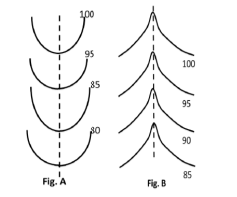
\includegraphics[width=0.7\textwidth]{Screenshot_2025_0818_132033.png}
	    \caption{}
    \label{fig:Q27}
    \end{figure}


    \hfill(GATE MN 2019)
\begin{enumerate}
\item Fig. A shows ridge and Fig. B shows valley
\item Fig. A shows anticline and Fig. B shows syncline
\item Fig. A shows syncline and Fig. B shows anticline
\item Fig. A shows valley and Fig. B shows ridge
\end{enumerate}


\item The availability of water in the root zone for plant use is maximum in the case of

	\hfill(GATE MN 2019)
\begin{multicols}{4}
\begin{enumerate}
\item sand
\item loam
\item clay
\item gravel
\end{enumerate}
\end{multicols}

  \item If the time to failure of a machine component is exponentially distributed, the reliability of the same at Mean Time To Failure (MTTF), (\textit{rounded off to three decimal places}), is \underline{\hspace{2cm}}.

	  \hfill(GATE MN 2019)

  \item The major and minor principal stresses at a point are 25 MPa and -5 MPa respectively. The maximum shear stress, in MPa at that point is \underline{\hspace{2cm}}.

	  \hfill(GATE MN 2019)

  \item For a function $f(x)$, $f(1)=5$ and $f''(1)=-5$. Ignoring all higher order terms in Taylor series, the value of the function at $x=1.01$ (\textit{rounded off to two decimal places}) is \underline{\hspace{2cm}}.

	  \hfill(GATE MN 2019)

  \item Proximate analysis of a coal sample gives 2.46\% moisture, 25.73\% volatile matter, and 42.89\% ash. The volatile matter of the coal sample, in percentage, on dry ash free (daf) basis (\textit{rounded off to two decimal places}) is \underline{\hspace{2cm}}.

	  \hfill(GATE MN 2019)

  \item A coarse sand aquifer has porosity 20\% and hydraulic conductivity $3.5 \times 10^{-3}$ m/s. If the hydraulic gradient is 0.00423 (m/m), then the average linear velocity of the groundwater in mm/s, (\textit{rounded off to three decimal places}) is \underline{\hspace{2cm}}.

	  \hfill(GATE MN 2019)

  \item In a slake durability test, mass of the drum with samples before the test and mass of the drum with oven-dried samples after the test are 1.52 kg and 1.48 kg respectively. If the mass of the drum is 1.05 kg, slake durability index of the sample, in percentage (\textit{rounded off to two decimal places}) is \underline{\hspace{2cm}}.

	  \hfill(GATE MN 2019)

  \item The ionic concentration of a mine water sample with pH close to 7.0 is given below. The alkalinity of the water expressed as equivalent CaCO$_3$, in mg/l, (\textit{rounded off to two decimal places}) is \underline{\hspace{2cm}}.
  
  \begin{table}[H]
    \centering\normalsize
  \begin{tabular}{|c|c|c|}
  \hline
  Cations & mg/l & Anions \\ \hline
  Ca$^{2+}$ & 95.0 & HCO$_3^-$ \\\hline
  \end{tabular}`
	  \caption{}
    \label{tab:Q35}
\end{table}


\hfill(GATE MN 2019)
	
\item From an elevated point A, when a stone is thrown vertically, it attains an upward velocity of $v$ at a height of $h$ from the point A. While falling, its downward velocity becomes $2v$ at a distance $h$ below the point A. The maximum height attained by the stone from point A is


	\hfill(GATE MN 2019)
\begin{multicols}{2}
\begin{enumerate}
  \item 5h/3
  \item 4h/3
  \item 6h/7
  \item 2h
\end{enumerate}
\end{multicols}


\item Water is pumped through a steel pipe of diameter 200 mm at a flow rate of 30 l/s. If the dynamic viscosity of water is $10^{-3}$ Pa·s, the Reynolds number of the flow is


	\hfill(GATE MN 2019)
\begin{multicols}{4}
\begin{enumerate}
  \item $2.83 \times 10^3$
  \item $2.83 \times 10^4$
  \item $1.91 \times 10^5$
  \item $1.91 \times 10^6$
\end{enumerate}
\end{multicols}


\item Matrix 
\[
\vec{A}=
\myvec{
0 & \beta & \gamma \\
\alpha & 0 & -\gamma \\
\alpha & -\beta & 0
}
\]
is orthogonal. The values of $\alpha, \beta$ and $\gamma$ respectively are

\hfill(GATE MN 2019)

\begin{multicols}{2}
\begin{enumerate}
  \item $\pm \sqrt{3}, \pm \sqrt{2}, \pm \sqrt{6}$
  \item $\pm \sqrt{6}, \pm \sqrt{3}, \pm \sqrt{2}$
  \item $\pm \sqrt{2}, \pm \sqrt{6}, \pm \sqrt{3}$
  \item $\pm \sqrt{2}, \pm \sqrt{3}, \pm \sqrt{6}$
\end{enumerate}
\end{multicols}

\item Match the following based on the equipment usage in a comminution circuit:



  \begin{table}[H]
    \centering\normalsize
\begin{tabular}{|c|c|}
\hline
\textbf{Equipment} & \textbf{Usage} \\ \hline
P. Gyratory crusher & 1. Secondary crushing \\ \hline
Q. Cone crusher     & 2. Grinding \\ \hline
R. Ball mill        & 3. Sizing \\ \hline
S. Grizzly          & 4. Primary crushing \\ \hline
\end{tabular}
\caption{}
    \label{tab:Q39}
\end{table}


\hfill(GATE MN 2019)
\begin{multicols}{2}
\begin{enumerate}
  \item P-1, Q-4, R-2, S-3  
  \item P-1, Q-2, R-3, S-4  
  \item P-4, Q-1, R-2, S-3  
  \item P-3, Q-1, R-4, S-2  
\end{enumerate}
\end{multicols}


\item Match the following for coal mining operation:

  \begin{table}[H]
    \centering\tiny

\begin{tabular}{|c|c|c|}
\hline
\textbf{Mining Method} & \textbf{Mode of Extraction} & \textbf{Loading/Conveying Equipment} \\ \hline
P. Longwall & A. Cutting by continuous miner & 1. AFC \\ \hline
Q. Mechanized bord and pillar & B. Drilling and blasting & 2. LHD \\ \hline
R. Semi-mechanized bord and pillar & C. Cutting by shearer & 3. Apron loader and gathering arm \\ \hline
S. Blasting gallery & D. Long hole drilling and blasting & 4. SDL \\ \hline
\end{tabular}
\caption{}
    \label{tab:Q40}
\end{table}


\hfill(GATE MN 2019)
\begin{multicols}{2}
\begin{enumerate}
  \item P-C-1, Q-D-3, R-A-2, S-B-4  
  \item P-C-1, Q-A-3, R-B-4, S-D-2  
  \item P-C-1, Q-A-4, R-B-3, S-D-2  
  \item P-B-3, Q-C-2, R-A-1, S-D-4  
\end{enumerate}
\end{multicols}



\item In the context of mine planning, match the following:

  \begin{table}[H]
    \centering\normalsize
\begin{tabular}{| m{6cm} | m{7cm} |}

\textbf{Technique / Algorithm} & \textbf{Preferred Application} \\

P. Lerchs–Grossman algorithm & 1. Ultimate pit limit \\
Q. Kriging & 2. Cut-off grade optimization \\
R. Lane’s theory & 3. Mine life \\
S. Taylor’s rule & 4. Reserve estimation \\

\end{tabular}

\caption{}
    \label{tab:Q41}
\end{table}

\hfill(GATE MN 2019)
\begin{multicols}{2}
\begin{enumerate}
\item P-4, Q-3, R-2, S-1
\item P-1, Q-2, R-3, S-4
\item P-1, Q-4, R-2, S-3
\item P-3, Q-2, R-4, S-1
\end{enumerate}
\end{multicols}


\item The figures shown represent the analysis of gas samples collected from a sealed off area in a coal mine over a period of time. The best representation of the progressive change of gaseous environment inside the sealed-off area is
\begin{figure}[H]
    \centering
        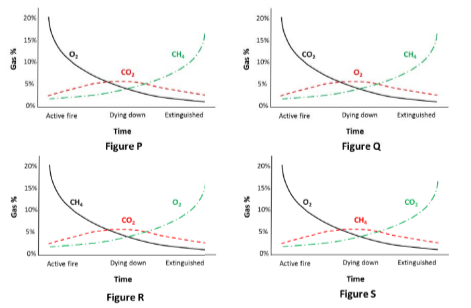
\includegraphics[width=1\textwidth]{Screenshot_2025_0818_150943.png}
	    \caption{}
    \label{fig:Q42}
    \end{figure}

    \hfill(GATE MN 2019)
\begin{multicols}{2}
\begin{enumerate}
\item Figure P
\item Figure Q
\item Figure R
\item Figure S
\end{enumerate}
\end{multicols}

\item The net annual cash flows for two small scale mining projects A and B are given below. The correct decision assuming 10\% discount rate as per NPV criterion is:


  \begin{table}[H]
    \centering\normalsize
\begin{tabular}{|c|c|c|}
\hline
Period in years & Project A (Rs. Cr) & Project B (Rs. Cr) \\
\hline
0 & -200 & -300 \\\hline
1 & 0 & 0 \\\hline
2 & 200 & 100 \\\hline
3 & 140 & 150 \\\hline
4 & 0 & 200 \\
\hline
\end{tabular}


\caption{}
    \label{tab:Q43}
\end{table}

\hfill(GATE MN 2019)
\begin{enumerate}
\item Project A is accepted but Project B is rejected
\item Projects A and B both are rejected
\item Project A is rejected but Project B is accepted
\item Projects A and B are both accepted but project A is better than project B
\end{enumerate}


\item Match the following features with the mining methods:

  \begin{table}[H]
    \centering\normalsize
\begin{tabular}{| m{6cm} | m{7cm} |}

\textbf{Features} & \textbf{Mining Method} \\

P. Ring Drilling & 1. Vertical crater retreat method \\
Q. Grizzly sublevel & 2. Sublevel stoping \\
R. Spherical charge blasting & 3. Underhand cut-and-fill stoping \\
S. Cemented hydraulic fill & 4. Block caving method \\
\end{tabular}
\caption{}
    \label{tab:Q44}
\end{table}

\hfill(GATE MN 2019)

\begin{multicols}{2}
\begin{enumerate}
\item P-2, Q-4, R-3, S-1
\item P-4, Q-3, R-2, S-1
\item P-2, Q-4, R-1, S-3
\item P-4, Q-3, R-1, S-2
\end{enumerate}
\end{multicols}


\item If area $S$, in the $x$–$y$ plane, is bounded by a triangle with vertices $(0,0)$, $(10,1)$ and $(1,1)$, the value of
\[
\iint_{S} \sqrt{x^2 - y^2} \, dx \, dy
\]
is \underline{\hspace{3cm}}.


\hfill(GATE MN 2019)
\item A double ended ranging drum shearer operates in a longwall retreating panel. The following data are provided:

  \begin{table}[H]
    \centering\normalsize
\begin{tabular}{ll}

Face length & 200 m \\
Web depth & 0.6 m \\
Cutting height & 2.5 m \\
Density of coal & 1.4 tonne/m$^3$ \\
Average cutting speed & 1.5 m/min \\
Average flitting speed & 4.0 m/min \\
Number of shifts/day & 3 \\

\end{tabular}

\caption{}
    \label{tab:Q46}
\end{table}
Method of cutting is unidirectional and each shift requires a non-operational time of 2.0 hours. The production per day in tonne (rounded off to one decimal place) is \underline{\hspace{3cm}}.


\hfill(GATE MN 2019)
\item In the linear programming problem,  
Maximize \[ Z = 48X_{1} + 36X_{2} \]  
Subject to:  
\[
\begin{aligned}
X_{1} &\leq 5 \\
X_{2} &\leq 8 \\
2X_{1} + \tfrac{4}{3}X_{2} &\leq 16 \\
X_{1} + X_{2} &= 10 \\
X_{1} &\geq 4 \\
X_{1}, X_{2} &\geq 0
\end{aligned}
\]  
The value of $Z$ is \underline{\hspace{2cm}}.  


\hfill(GATE MN 2019)

\item A shovel operates 300 days in a year, 2 shifts in a day, and 4 hours in a shift to achieve the target production of 30 Million tonne per annum. The following parameters relate to the loading operations:  


\begin{enumerate}
\item Bucket capacity of shovel : 15 m$^{3}$
\item Shovel cycle time : 44 s
\item Bucket fill factor : 0.85
\item Bulk density of the muck : 3.00 tonne/m$^{3}$
\end{enumerate}


The minimum number of shovels required to achieve the production is \underline{\hspace{2cm}}. 

\hfill(GATE MN 2019)


\item A set of tubs is pulled by a 15 tonne diesel locomotive at a gradient of 1 in 100 with an acceleration of 0.05 m/s$^{2}$. The coefficient of adhesion between the wheel and the track is 0.2 and the frictional resistance coefficient is 0.01. The maximum mass, in tonne, the locomotive can pull (rounded off to one decimal place) is \underline{\hspace{2cm}}.  


	\hfill(GATE MN 2019)
\item The characteristic curves of two mine fans installed in series in a fan drift are  
\[
P = 2000 - 60Q - 0.02Q^{2} \quad \text{and} \quad P = 3000 - 80Q - 0.02Q^{2}
\]  
where $P$ is pressure in Pa and $Q$ is quantity in m$^{3}$/s. If the mine quantity is 70 m$^{3}$/s, the mine resistance, in Ns$^{2}$/m$^{8}$, (rounded off to two decimal places) is \underline{\hspace{2cm}}.  

\hfill(GATE MN 2019)


\item Three equipment A, B, and C located side by side and operating simultaneously produce a sound power level of 77.5 dB. The sound power levels of A and B are 68 dB and 70 dB respectively. The sound power level of C (rounded off to one decimal place) in dB, is \underline{\hspace{2cm}}.  


	\hfill(GATE MN 2019)

\item The main surface fan of a mine has characteristic curve approximated by  
\[
P = 1700 - 10Q
\]  
where $P$ is pressure in Pa and $Q$ is quantity in m$^{3}$/s. A booster fan is installed in section A such that there is no air flow in section B. The operating pressure of the main surface fan, in Pa, (rounded off to two decimal places) is \underline{\hspace{2cm}}.

\begin{figure}[H]
    \centering
        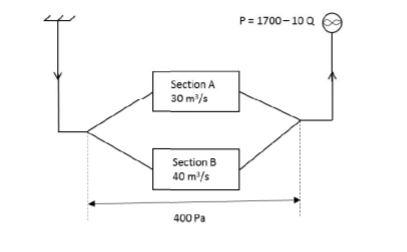
\includegraphics[width=0.7\textwidth]{Screenshot_2025_0818_152006.png}
	    \caption{}
    \label{fig:Q53}
    \end{figure}


    \hfill(GATE MN 2019)

\item Two points A and B are located 150 m apart in the East-West orientation on the bank of a river as shown in the figure. Considering a station C on the north bank the bearings of AC and BC are observed to be 42$^{\circ}$ and 335$^{\circ}$ respectively. The width of the river, in m, (rounded off to two decimal places) is \underline{\hspace{2cm}}.  
\begin{figure}[H]
    \centering
        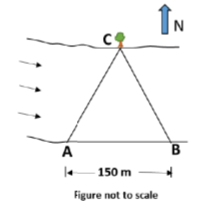
\includegraphics[width=0.6\textwidth]{Screenshot_2025_0818_152607.png}
	    \caption{}
    \label{fig:Q54}
    \end{figure}



    \hfill(GATE MN 2019)
\item If $x = 3^{1/3} + 3^{-1/3}$, the value of $3x^{3} - 9x - 10$ is \underline{\hspace{2cm}}.  


	\hfill(GATE MN 2019)

\item A pump delivers 3000 liter of water in 2.0 minutes through a pipe of length 1000 m laid on a gradient of 1 in 10. The combined efficiency of pump and motor is 70\%. If friction and shock losses are negligible, the input power to the motor in kW (rounded off to one decimal place) is \underline{\hspace{3cm}}.


	\hfill(GATE MN 2019)

\item A sand water slurry of specific gravity 1.45 contains sand of grain density 2.6 g/cc. The weight percent of sand in the slurry (rounded off to two decimal places) is \underline{\hspace{3cm}}.


	\hfill(GATE MN 2019)

\item For a mining company the unit transportation cost from a mine to a washery, and supply and demand are shown below:

\begin{table}[H]
\centering
\begin{tabular}{|c|c|c|c|c|c|}
\hline
\multirow{2}{*}{Mine} & \multicolumn{4}{c|}{Washery} & \multirow{2}{*}{Supply} \\ \cline{2-5}
 & A & B & C & D & \\ \hline
M1 & 30 & 0  & 40 & 20 & 500 \\ \hline
M2 & 24 & 16 & 22 & 40 & 700 \\ \hline
M3 & 0  & 32 & 28 & 36 & 800 \\ \hline
Demand & 300 & 400 & 600 & 700 & \\ \hline
\end{tabular}
	\caption{}
	\label{tab:Q57}
\end{table}


The total cost of transportation using the Vogel’s approximation method is \underline{\hspace{3cm}}.


\hfill(GATE MN 2019)

\item In a bord and pillar panel, 6 square pillars are developed as shown in the figure below. The depth of the seam is 300 m and the average unit weight of overburden rock is 25 kN/m$^3$. If the pillar strength is 15 MPa, the safety factor of the shaded pillar zone (rounded off to two decimal places) is \underline{\hspace{3cm}}.


\begin{figure}[H]
    \centering
        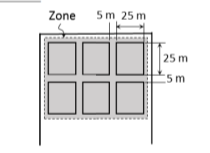
\includegraphics[width=0.5\textwidth]{Screenshot_2025_0818_154544.png}
	    \caption{}
    \label{fig:Q58}
    \end{figure}


    \hfill(GATE MN 2019)
\item Water enters a sump having the shape of an inverted frustum at a rate of 500 m$^3$/h. The sump is initially filled up to 2.0 m height. The time taken in days to fill the remaining part of the sump (rounded off to one decimal place) is \underline{\hspace{3cm}}.


\begin{figure}[H]
    \centering
        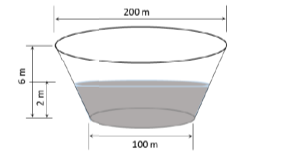
\includegraphics[width=0.6\textwidth]{Screenshot_2025_0818_154255.png}
	    \caption{}
    \label{fig:Q59}
    \end{figure}


    \hfill(GATE MN 2019)
\item The uniaxial stress-strain behavior of a rock sample is shown in the figure. The elastic modulus is $E = 20,000$ MPa. If $\varepsilon_p$ is the plastic strain, the value of the damage parameter $D$ (rounded off to two decimal places) is \underline{\hspace{3cm}}.


\begin{figure}[H]
    \centering
	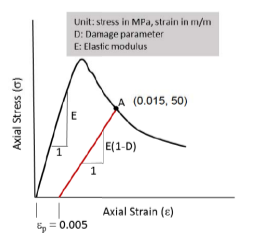
\includegraphics[width=0.6\textwidth]{Screenshot_2025_0818_153819.png}
	    \caption{}
    \label{fig:Q60}
    \end{figure}

    \hfill(GATE MN 2019)
\item The insitu stress field around a circular tunnel is shown in the figure. Points A and B are located at the boundary of the tunnel. If the tangential stress at Point A is 3 times that of at Point B, the value of insitu stress ratio, $k$, is \underline{\hspace{3cm}}.


\begin{figure}[H]
    \centering
        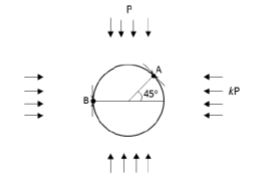
\includegraphics[width=0.6\textwidth]{Screenshot_2025_0818_153102.png}
	    \caption{}
    \label{fig:Q61}
    \end{figure}

    

    \hfill(GATE MN 2019)
\item Data related to explosive and blasthole are given below. Assuming 1 kcal to be 4.2 kJ, the power of explosive in GW in the blasthole (\textit{round off to one decimal place}) is \underline{\hspace{2cm}}. 

\begin{table}[H]
\centering
\begin{tabular}{l l}
Diameter of the borehole   & : 200 mm \\
Charge length              & : 8 m \\
Density of ANFO            & : 0.8 g/cc \\
Heat of explosion          & : 912 cal/g \\
VOD                        & : 4500 m/s \\
Initiation                 & : Bottom \\
\end{tabular}
\caption{}
	\label{tab:Q62}
\end{table}


\hfill(GATE MN 2019)
\item A rock block of mass 100 kg is to be lifted by a horizontal force $P$ as shown in the figure below. Smooth rollers are placed between the wedges. The coefficient of static friction between wedge A and surface C and between wedge B and surface D is 0.3. Ignoring the weight of the wedges and the friction between the roller and the wedges, the minimum force $P$ in kg required to lift the block (\textit{round off to one decimal place}) is \underline{\hspace{2cm}}. 


\begin{figure}[H]
    \centering
	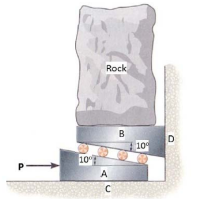
\includegraphics[width=0.6\textwidth]{Screenshot_2025_0818_160753.png}
	    \caption{}
    \label{fig:Q63}
    \end{figure}

    \hfill(GATE MN 2019)
\item A joint plane dipping at $30^\circ$ intersects the slope edge and the crest as shown in the figure below. The unit weight of rock is 25 kN/m$^3$, and cohesion and friction angle of the joint surface are 40 kPa and $25^\circ$ respectively. The safety factor of the shaded block (\textit{round off to two decimal places}) is \underline{\hspace{2cm}}.

\begin{figure}[H]
    \centering
	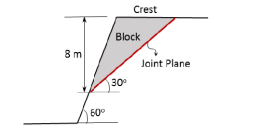
\includegraphics[width=0.6\textwidth]{Screenshot_2025_0818_155710.png}
	    \caption{}
    \label{fig:Q64}
    \end{figure}

\hfill(GATE MN 2019)
\item The random variable $X$ has probability density function as given by
\[
f(x) = 
\begin{cases}
3x^2, & 0 \leq x \leq 1 \\
0, & \text{otherwise}
\end{cases}
\]

The value $E(X^2)$ (\textit{rounded off to one decimal place}) is \underline{\hspace{2cm}}.


\hfill(GATE MN 2019)

\end{enumerate}
\begin{center}
\huge{END OF QUESTION PAPER}
\end{center}

\end{document}

